\chapter{Lecture 13}

\section*{Intrinsic characterization of $\mathscr{H}$}\pageoriginale

$\mathscr{H}$, considered as a topological vector space, is
intrinsically attached to the manifold \iec $\mathscr{H}$ is
independent of the Riemannian metric. We shall now give an intrinsic
characterization of $\mathscr{H}$.

Suppose $U$ is the domain of a local coordinate system
$x_{1},\ldots,x_{N}$ and $K$ a compact set contained in $U$. Suppose
$\omega$ is a measurable $p$ form such that
$(\omega,\omega)<\infty$. Suppose
$$
\omega=\sum \omega_{I}dx_{I}
$$
on $U$. ($I$ is a system of $p$ indices written in the increasing
order). Let further
$$
(\omega,\omega)_{a}=\sum g^{IJ}(a)\omega_{I}(a)\omega_{J}(a).
$$
If $m(a)$ is the smallest eigen value of the matrix $(g^{IJ}(a))$,
$m(a)$ is a continuous function in $K$ and hence has a lower bound $m_1$
in $K$; $m_{1}>0$, since $(g^{IJ}(a))$ are positive definite. Since,
$$
\sum_{I,J}g^{IJ}(a)\omega_{I}(a)\omega_{J}(a)\geq
m(a)\sum_{I,J}[\omega_{I}(a)]^{2} 
$$
it follows that
\begin{align*}
(\omega,\omega) &\geq
  \int\limits_{K}\left(\sum_{I,J}g^{IJ}\omega_{I}\omega_{J}\right)\sqrt{g}dx_{1}\ldots
  dx_{N}\\
&\geq Cm_{1}\int\limits_{K}\sum |\omega_{I}|^{2}dx_{1}\ldots dx_{N}
\end{align*}
where $C\geq 0$ is the lower bound of $\sqrt{g}$ in $K$. Thus, if
$(\omega,\omega)<\infty$, 
$$
\int\limits_{K}\sum|\omega_{I}|^{2}dx_{1}\ldots dx_{N}<\infty.
$$\pageoriginale

Conversely, suppose $\omega$ is a measurable $p$-form such that for
every compact $K$ contained in the domain $U$ of a map
$$
\int\limits_{K}\sum|\omega_{I}|^{2}dx_{1}\ldots dx_{N}<\infty;
$$
then $(\omega,\omega)<\infty$. We choose a finite covering of the
manifold by domains $U_{\lambda}$ of maps and a partition of unity
$\{\alpha_{\lambda}\}$ subordinate to the covering $U_{\lambda}$. Let
$K_{\lambda}$ be the support of $\alpha_{\lambda}$. Then, with the
obvious notation,
\begin{align*}
(\omega,\omega) &= \int\limits_{V}(\omega,\omega)_{a}\tau\\
&=
  \sum_{\lambda}\int\limits_{V}(\omega,\omega)_{a}\alpha_{\lambda}\tau\\
&=
  \sum_{\lambda}\int\limits_{U_{\lambda}}(\omega,\omega)_{a}\alpha_{\lambda}\tau\\
&=
  \sum_{\lambda}\int\limits_{U_{\lambda}}g^{IJ}(a)^{(\lambda)}\omega^{(\lambda)}_{I}\omega^{(\lambda)}_{J}\alpha_{\lambda}\sqrt{g}^{(\lambda)}dx^{(\lambda)}_{1}\ldots
  dx_{N}^{(\lambda)}.
\end{align*}
Let $M_{\lambda}(a)$ be the greatest eigenvalue of
$(g^{IJ}(a)^{(\lambda)})$. The functions $M_{\lambda}$,
$\alpha_{\lambda}$ and $\sqrt{g}^{(\lambda)}$ are bounded in
$K_{\lambda}$ so that
\begin{align*}
(\omega,\omega) &\leq \sum
  c_{\lambda}\int\limits_{K_{\lambda}}
  \left(\sum|\omega_{I}^{(\lambda)}|^{2}\right) dx^{(\lambda)}_{1}\ldots
  dx^{(\lambda)}_{N},C_{\lambda}\text{ \ a constant,}\\
&<\infty. 
\end{align*}

Thus\pageoriginale the elements of $\mathscr{H}$ can be characterized
as classes, a class being the set of all measurable forms almost
everywhere equal to a form whose coefficients are square summable on
every compact set contained in the domain of a map.

A simple application of the Fisher-Riesz theorem would now show that
$\mathscr{H}$ is complete.

It may be remarked convergence in $\mathscr{H}$ implies convergence in
$\mathscr{D}'$. 

\section*{Decomposition of $\mathscr{H}$}

We shall now decompose the space $\mathscr{H}$ into the direct sum of
three fundamental spaces which are mutually orthogonal. Let
$\mathscr{H}_{1}$ be the subspace of the elements $\omega\in
\mathscr{H}$ such that $\Delta\omega=0$ (in the sense of currents). It
follows from the elliptic character of $\Delta$ that $\mathscr{H}_{1}$
is exactly the space of harmonic forms. Since $d$ and $\partial$ are
continuous operators on currents, $\mathscr{H}_{1}$ is closed. In fact
we shall see later that $\mathscr{H}_{1}$ is finite dimensional.
\begin{figure}[H]
\centering
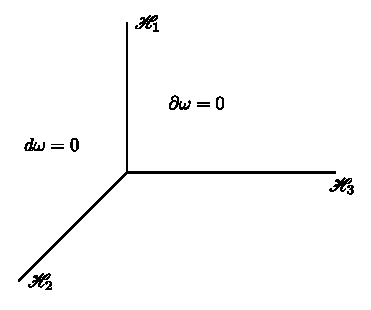
\includegraphics{schwartz-fig1.eps}
\end{figure}
We\pageoriginale define $\mathscr{H}_{2}$ to be the space of elements
$\omega\in \mathscr{H}$ such that $(\omega,\ast\varphi)=0$ for every
$\varphi\in \mathscr{D}$ with $\partial\varphi=0$. $\mathscr{H}_{2}$
is a closed subspace because of the continuity of the scalar
product. We shall now give another interpretation of the space
$\mathscr{H}_{2}$. If $\omega\in
\mathscr{H}_{2}$ then $\langle \omega,\ast\varphi\rangle=0$ for every
$\ast\varphi$ such that $d(\ast\varphi)=0$ or $\omega$ is orthogonal
to all $N-p$ forms which are closed. By the orthogonality theorem
$\omega$ is the coboundary of a current. Now let
$\widetilde{\mathscr{H}}$ be the subspace of elements $\omega$ of
$\mathscr{H}$ for which $d\omega\in \mathscr{H}$ (the $\mathscr{H}$'s
have different degrees). Then $d$ operates on
$\widetilde{\mathscr{H}}$ and this gives a cohomology. There is a
natural homomorphism of $H(\widetilde{\mathscr{H}})$ into
$H(\mathscr{D}')$. Another de Rham's theorem states that this
homomorphism is an isomorphism onto. This implies, in particular, that
if $\omega\in\mathscr{H}$ is the coboundary of a current it is also
the coboundary of an element
$\widetilde{\omega}\in\widetilde{\mathscr{H}}$. So $\mathscr{H}_{2}$
is the space of forms of $\mathscr{H}$ which are coboundaries of forms
of $\mathscr{H}$: 
$$
\mathscr{H}_{2}=d\mathscr{H}\cap \mathscr{H}.
$$

We define $\mathscr{H}_{3}$ to be the space of elements
$\omega\in\mathscr{H}$ such that $(\omega, \varphi)=0$ for every
$\varphi\in \mathscr{D}$ with $d\varphi=0$. $\mathscr{H}_{3}$ is
closed. If $\omega\in \mathscr{H}_{3}$, $\ast\omega\in\mathscr{H}_{2}$
and therefore $=\partial \widetilde{\omega}$,
$\widetilde{\omega}\in\mathscr{H}$. So $\mathscr{H}_{3}$ is the space
of forms of $\mathscr{H}$ which are star coboundaries of forms of
$\mathscr{H}$: 
$$
\mathscr{H}_{3}=\partial \mathscr{H}\cap \mathscr{H}.
$$

We shall prove that $\mathscr{H}_{1}$, $\mathscr{H}_{2}$ and
$\mathscr{H}_{3}$ are mutually orthogonal\pageoriginale. Suppose
$\alpha\in\mathscr{H}_{1}$ and $\beta\in \mathscr{H}_{2}$. Then
\begin{align*}
(\alpha,\beta) &=
  (\alpha,d\widetilde{\omega}),\widetilde{\omega}\in\mathscr{H}\\
&= (\partial\alpha,\widetilde{\omega})\text{ since } \alpha \text{ is
    a }C^{\infty}\text{ form}\\
&=0\text{\quad as } \partial\alpha=0.
\end{align*}
Similarly $\mathscr{H}_{1}$ and $\mathscr{H}_{3}$ are orthogonal. To
prove that $\mathscr{H}_{2}$ and $\mathscr{H}_{3}$ are orthogonal we
shall first prove that
$$
\mathscr{H}_{2}=\ob{d\mathscr{D}}\quad\text{and}\quad
\mathscr{H}_{3}=\ob{\partial\mathscr{D}} 
$$

Evidently $d\mathscr{D}\subset \mathscr{H}_{2}$ and as
$\mathscr{H}_{2}$ is closed $\ob{d\mathscr{D}}\subset
\mathscr{H}_{2}$. If $\mathscr{H}_{2}\neq \ob{d\mathscr{D}}$ as
$\mathscr{H}_{2}$ is a closed subspace we can find a vector
$\lambda\in \mathscr{H}_{2}$, $\lambda\neq 0$ such that $\lambda$ is
orthogonal to $d\mathscr{D}$ or $(\lambda,d\varphi)=0$ for every
$\varphi\in\mathscr{D}$ or $(\partial\lambda,\varphi)=0$ for every
$\varphi\in\mathscr{D}$. This implies that
$\partial\lambda=0$. Already $d\lambda=0$ since $\lambda$ is
derived. So $\lambda\in\mathscr{H}_{1}$ and
$\lambda\in\mathscr{H}_{2}$. As $\mathscr{H}_{1}$ and
$\mathscr{H}_{2}$ are orthogonal $\lambda=0$; this proves
$\mathscr{H}_{2}=\ob{d\mathscr{D}}$. Similarly
$\mathscr{H}_{3}=\ob{\partial \mathscr{D}}$. If $\alpha$,
$\beta\in\mathscr{D}$ 
$$
(d\alpha,\partial\beta)=(dd\alpha,\beta)=0
$$
\iec $d\mathscr{D}$ and $\partial \mathscr{D}$ are orthogonal. Since
$\ob{d\mathscr{D}}=\mathscr{H}_{2}$ and
$\ob{\partial\mathscr{D}}=\mathscr{H}_{3}$ it follows that
$\mathscr{H}_{2}$ and $\mathscr{H}_{3}$ are orthogonal.

We next show that $\mathscr{H}_{1}$, $\mathscr{H}_{2}$ and
$\mathscr{H}_{3}$ span $\mathscr{H}$. Suppose $\omega$ is orthogonal
to $\mathscr{H}_{2}$ and $\mathscr{H}_{3}$; then $(\omega,d\alpha)=0$
for every $\alpha\in\mathscr{D}$ or $(\partial\omega,\alpha)=0$ for
every $\alpha\in \mathscr{D}$ or $\partial \omega=0$; similarly
$d\omega=0$. Hence $\omega\in\mathscr{H}_{1}$. This proves that 
$$
\mathscr{H}=\mathscr{H}_{1}+\mathscr{H}_{2}+\mathscr{H}_{3}.
$$\pageoriginale
We denote by $\pi_{1}$, $\pi_{2}$ and $\pi_{3}$ the projections on
$\mathscr{H}_{1}$, $\mathscr{H}_{2}$ and $\mathscr{H}_{3}$
respectively.

$\mathscr{H}_{1}+\mathscr{H}_{2}$ is the orthogonal of
$\mathscr{H}_{3}$ or $\partial\mathscr{D}$, so
$\mathscr{H}_{1}+\mathscr{H}_{2}$ is the space of forms $\omega$ with
$d\omega=0$ (in the sense of the
currents). $\mathscr{H}_{1}+\mathscr{H}_{3}$ is the space of forms
$\omega$ with $\partial\omega=0$ and $\mathscr{H}_{2}+\mathscr{H}_{3}$
is the space of forms orthogonal to the space of harmonic forms.

\section*{Cohomology and harmonic forms. Hodge's theorem}

In every cohomology class of $C^{\infty}$ forms there exists one and
only one harmonic form. Let $\omega$ be a representative of the
cohomology class;
$\omega\in\mathscr{H}_{1}+\mathscr{H}_{2}$. $\pi_{1}\omega$ is a
harmonic form and $\pi_{2}\omega$ which is the coboundary of a current
is the coboundary of a form by de Rham's theorem. As
$$
\omega-\pi_{1}\omega=\pi_{2}\omega
$$
$\omega$ and $\pi_{1}\omega$ are cohomologous. So $\pi_{1}\omega$ is a
harmonic form belonging to the class of $\omega$. If $\omega_{1}$ and
$\omega_{2}$ are two harmonic forms in the same cohomology class,
$\omega_{1}-\omega_{2}\in\mathscr{H}_{1}\cap \mathscr{H}_{2}=0$ or
$\omega_{1}=\omega_{2}$. Thus we have, in fact, a canonical
isomorphism between the cohomology space of $C^{\infty}$ forms and the
space of harmonic forms. The dimension of the space of harmonic forms
of degree $p$ is the $p$th Betti number of the manifold which is
finite by the third part of de Rham's theorem.

Suppose $\omega\in\mathscr{H}_{2}$; then $\omega=d\widetilde{\omega}$,
$\widetilde{\omega}\in\mathscr{H}$. 
There\pageoriginale is one and only one choice of the primitive
$\widetilde{\omega}$ which belongs to $\mathscr{H}_{3}$. For, if
$\omega=d\theta$, $\theta\in\mathscr{H}$ put
$\widetilde{\omega}=\pi_{3}\theta$; then
$\omega=d\widetilde{\omega}$. If
$\omega=d\widetilde{\omega}_{1}=d\widetilde{\omega}_{2}$,
$\widetilde{\omega}_{1}$, $\widetilde{\omega}_{2}\in \mathscr{H}_{3}$,
$d(\widetilde{\omega}_{1}-\widetilde{\omega}_{2})=0$, which implies
that
$\widetilde{\omega}_{1}-\widetilde{\omega}_{2}\in\mathscr{H}_{3}\cap
\mathscr{H}_{2}$ so that
$\widetilde{\omega}_{1}=\widetilde{\omega}_{2}$. 

Similarly any element of $\mathscr{H}_{3}$ is the star coboundary of
one and only one element of $\mathscr{H}_{2}$. In both the cases the
choice of the unique primitive is linear but not yet continuous.

Now let $\omega\in\mathscr{H}_{2}$; $\omega=d\theta$,
$\theta\in\mathscr{H}_{3}$. But $\theta=\partial\widetilde{\omega}$,
$\widetilde{\omega}\in\mathscr{H}_{2}$. Consequently for every
$$
\omega\in\mathscr{H}_{2},\omega=d\partial\widetilde{\omega},\widetilde{\omega}\in\mathscr{H}_{2}. 
$$
This $\widetilde{\omega}$ is unique. Every element $\omega$ of
$\mathscr{H}_{2}$ is thus expressed in one and only one way in the
form
$$
\omega=d\partial
\widetilde{\omega},\widetilde{\omega}\in\mathscr{H}_{2}.
$$
However, for $\omega\in \mathscr{H}_{2}$, $\partial d\omega=0$ so that
$d\partial =-\Delta$. So any form $\omega\in\mathscr{H}_{2}$ can be
written uniquely in the form
$$
\omega=-\Delta\widetilde{\omega},\widetilde{\omega}\in\mathscr{H}_{2}.
$$
Similarly every form in $\mathscr{H}_{3}$ is uniquely expressible as
the Laplacian of an element of $\mathscr{H}_{3}$. As a consequence
every form orthogonal to all the harmonic forms is the Laplacian of
one and only one element of
$\mathscr{H}_{2}+\mathscr{H}_{3}$. Conversely if $\omega$ is the
Laplacian of an element, then it belongs to
$\mathscr{H}_{2}+\mathscr{H}_{3}$. 

We\pageoriginale have thus completely solved the equations $dX=A$,
$\partial X=A$ and $\Delta ~X=A$ in $\mathscr{H}$. The equation $dX=A$
is solvable if 
$A\in\mathscr{H}_{2}$. If $A\in\mathscr{H}_{2}$ there exists a unique
solution $X\in\mathscr{H}_{3}$. Any general solution is given by
$X=X_{0}+$ closed form. The equation $\partial X=A$ is solvable if
$A\in\mathscr{H}_{3}$ and there exists a unique solution
$X_{0}\in\mathscr{H}_{2}$. A general solution is obtained by
$X=X_{0}+$ closed form. The equation $\Delta X=A$ is solvable if
$A\in\mathscr{H}_{2}+\mathscr{H}_{3}$; there exists a unique solution
orthogonal to the space of harmonic forms and a general solution is
obtained by adding to this particular solution any harmonic
form. These results constitute Hodge's theorem.


